\documentclass[a4paper]{article}

\usepackage{fullpage} % Package to use full page
\usepackage{parskip} % Package to tweak paragraph skipping
\usepackage{amsmath}
\usepackage{hyperref}
\usepackage{amsmath,amsfonts,amsthm} % Math packages
\usepackage{graphicx}
\usepackage{listings}
\usepackage{color}
\usepackage{float}
\definecolor{keywords}{RGB}{255,0,90}
\definecolor{comments}{RGB}{0,0,113}
\definecolor{red}{RGB}{160,0,0}
\definecolor{green}{RGB}{0,150,0}
\definecolor{codegreen}{rgb}{0,0.6,0}
\definecolor{codegray}{rgb}{0.5,0.5,0.5}
\definecolor{codepurple}{rgb}{0.58,0,0.82}
\definecolor{backcolour}{rgb}{0.95,0.95,0.92}
\definecolor{brown}{rgb}{0.59, 0.29, 0.0}
\definecolor{beaublue}{rgb}{0.74, 0.83, 0.9}
\definecolor{orange}{rgb}{1.0, 0.5, 0.0}
\definecolor{darkslategray}{rgb}{0.18, 0.31, 0.31}
\definecolor{deepblue}{rgb}{0,0,0.5}
\definecolor{deepred}{rgb}{0.6,0,0}
\definecolor{deepgreen}{rgb}{0,0.5,0}
\lstdefinestyle{myMatlabstyle}{
	language=Matlab,
	backgroundcolor=\color{white},   
	commentstyle=\color{codegreen},
	keywordstyle=\color{blue},
	identifierstyle=\color{brown},
	numberstyle=\tiny\color{codegray},
	stringstyle=\color{orange},
	basicstyle=\footnotesize,
	breakatwhitespace=false,         
	breaklines=true,                 
	captionpos=b,                    
	keepspaces=true,                 
	numbers=left,                    
	numbersep=5pt,                  
	showspaces=false,                
	showstringspaces=false,
	showtabs=false,                  
	tabsize=2
}
\lstdefinestyle{myPythonstyle}{
	language=Python, 
	basicstyle=\ttfamily\small, 
	keywordstyle=\color{keywords},
	commentstyle=\color{comments},
	stringstyle=\color{red},
	showstringspaces=false,
	identifierstyle=\color{green},
}
\lstset{language=Matlab,frame=single}
\lstset{language=Python,frame=single}
\title{AMATH 522: Problem Set 3}
\author{Jithin D. George}
%\date{7/11/16}

\begin{document}

\maketitle
\section{Coupled Oscillators}
The coupled oscillators are modeled by the differential equations written below.
\begin{lstlisting}[style=MyMatlabstyle]
function deriv = coup_osc(tspan ,y,dummy, g,p)


%Differntial Equations
dy = zeros(12,1);

%First Oscillator
dy(1) = -y(1) + p(1)/(1.+y(6)^p(4))+ p(2);
dy(2) = -y(2) + p(1)/(1.+y(4)^p(4))+ p(2);
dy(3) = -y(3) + p(1)/(1.+y(5)^p(4))+ p(2);
dy(4) = -p(3)*(y(4)-y(1))+g*(y(10)-y(4));
dy(5) = -p(3)*(y(5)-y(2))+g*(y(11)-y(5));
dy(6) = -p(3)*(y(6)-y(3))+g*(y(12)-y(6));

%Second Oscillator
dy(7) = -y(7) + p(1)/(1.+y(12)^p(4))+ p(2);
dy(8) = -y(8) + p(1)/(1.+y(10)^p(4))+ p(2);
dy(9) = -y(9) + p(1)/(1.+y(11)^p(4))+ p(2);
dy(10) = -p(3)*(y(10)-y(7))+g*(y(4)-y(10));
dy(11) = -p(3)*(y(11)-y(8))+g*(y(5)-y(11));
dy(12) = -p(3)*(y(12)-y(9))+g*(y(6)-y(12));

deriv=dy;
\end{lstlisting}
We solve them in Matlab using ode45.
\begin{lstlisting}[style=MyMatlabstyle]
%Repressilator

clc; clear all; close all;
init = rand(12,1);
tspan=[0 200];

alpha=50;

alpha0=0;
beta=0.2;
n=2;
p = [alpha,alpha0,beta,n];

%Uncoupled Oscillations

[t,Y] = ode45('coup_osc',tspan,init,[],0,p);

figure(1)
set(gca,'FontSize',16)
plot3(Y(:,1),Y(:,3),Y(:,5),'g',Y(:,7),Y(:,9),Y(:,11),'LineWidth',3) ; 
legend('m lalcl','m2 lalcl')


figure(2)
set(gca,'FontSize',16)
plot(t,Y(:,1:3),'LineWidth',3) ; hold on;
plot(t,Y(:,4:6),:,'LineWidth',3) ; hold on;
plot(t,Y(:,7:9),'LineWidth',3) ; hold on;
plot(t,Y(:,10:12),:,'LineWidth',3) ; hold off;
legend('m lalcl','p lacl','m tetR','p tetR','m cl','p cl','m2 lalcl','p2 lacl','m2 tetR','p2 tetR','m2 cl','p2 cl')

figure(3)
set(gca,'FontSize',16)
plot(t,Y(:,1),'LineWidth',3) ; hold on;
plot(t,Y(:,7),'g','LineWidth',3) ; hold off;
legend('m lalcl','m2 lalcl')
xlabel('t') ; 

%Coupled Oscillations

[t,Y] = ode45('coup_osc',tspan,init,[],10,p);

figure(4)
set(gca,'FontSize',16)
plot3(Y(:,1),Y(:,3),Y(:,5),'g',Y(:,7),Y(:,9),Y(:,11),'LineWidth',3) ; 
legend('m lalcl','m2 lalcl')


figure(5)
set(gca,'FontSize',16)
plot(t,Y(:,1:3),'LineWidth',3) ; hold on;
plot(t,Y(:,4:6),:,'LineWidth',3) ; hold on;
plot(t,Y(:,7:9),'LineWidth',3) ; hold on;
plot(t,Y(:,10:12),:,'LineWidth',3) ; hold off;
legend('m lalcl','p lacl','m tetR','p tetR','m cl','p cl','m2 lalcl','p2 lacl','m2 tetR','p2 tetR','m2 cl','p2 cl')


figure(6)
set(gca,'FontSize',16)
plot(t,Y(:,1),'LineWidth',3) ; hold on;
plot(t,Y(:,7),'g','LineWidth',3) ; hold off;
legend('m lalcl','m2 lalcl')
xlabel('t') ; 
\end{lstlisting}

 	   \begin{figure}[H]
 	   	\centering
 	   	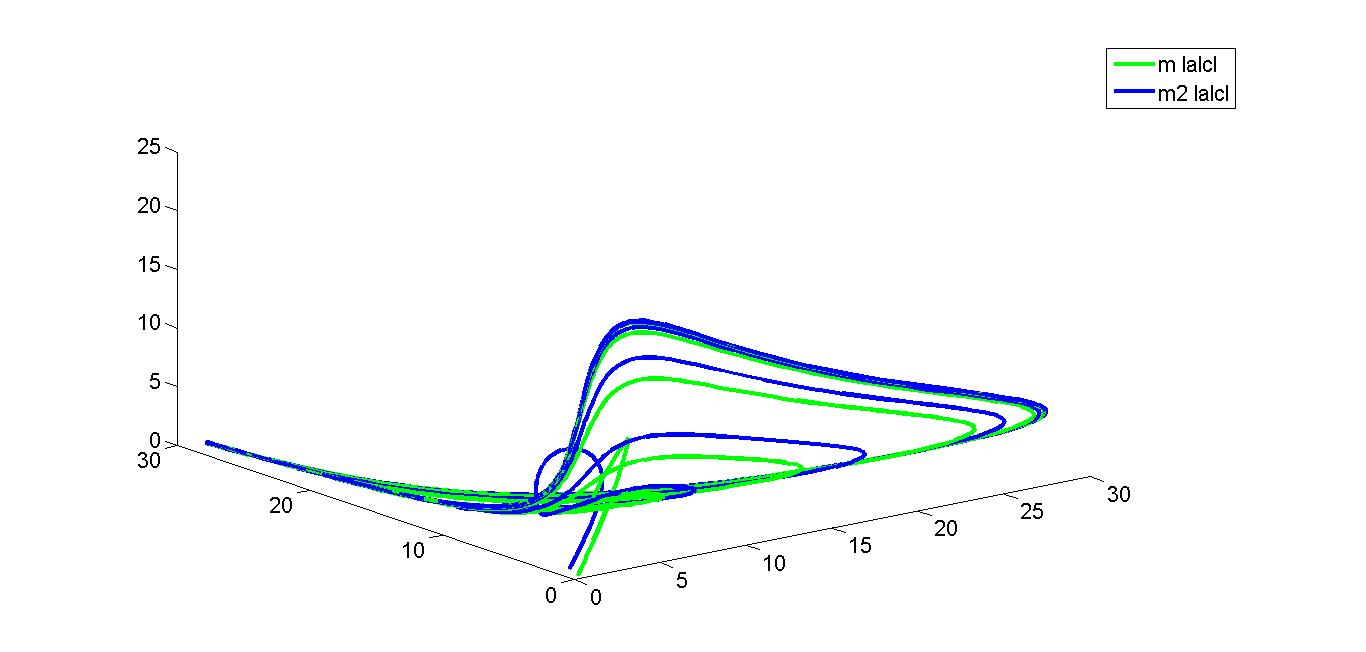
\includegraphics[width=12cm]{uncoup3d}
 	   	\caption{The uncoupled case }
 	   \end{figure}
 	   \begin{figure}[H]
 	   	\centering
 	   	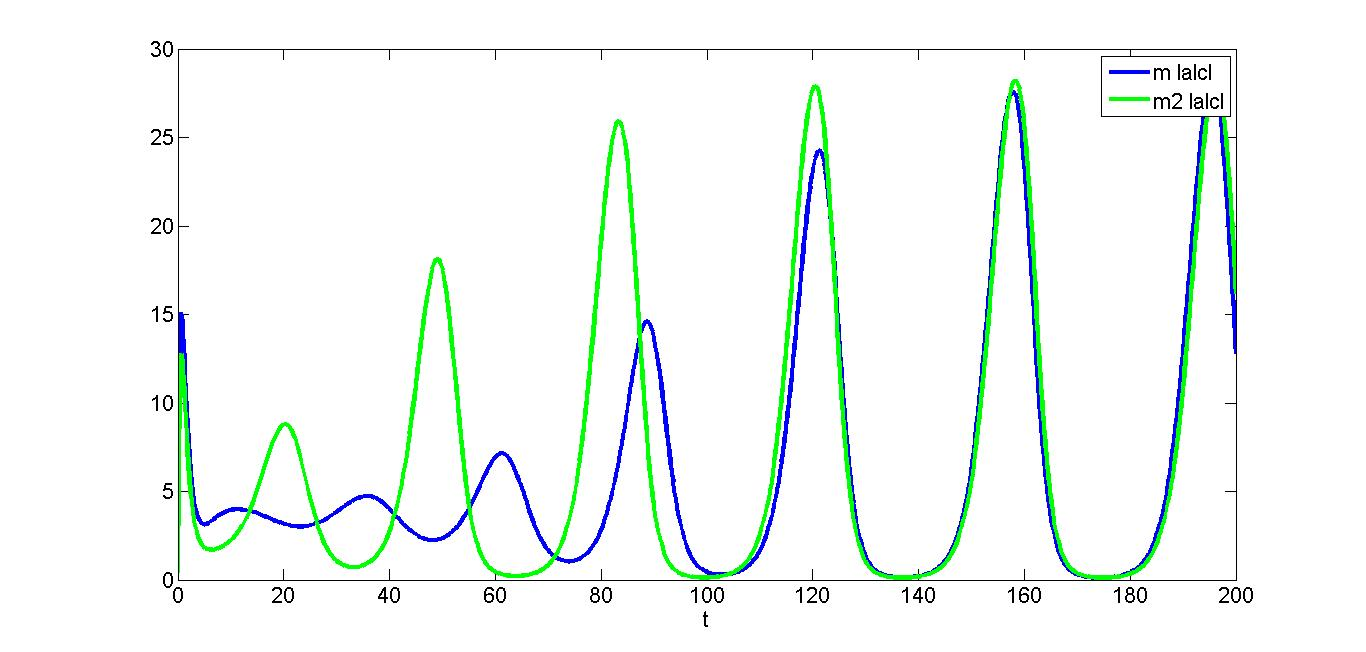
\includegraphics[width=12cm]{uncouposc}
 	   	\caption{Oscillations in the uncoupled case}
 	   \end{figure} 
 	   \begin{figure}[H]
 	   	\centering
 	   	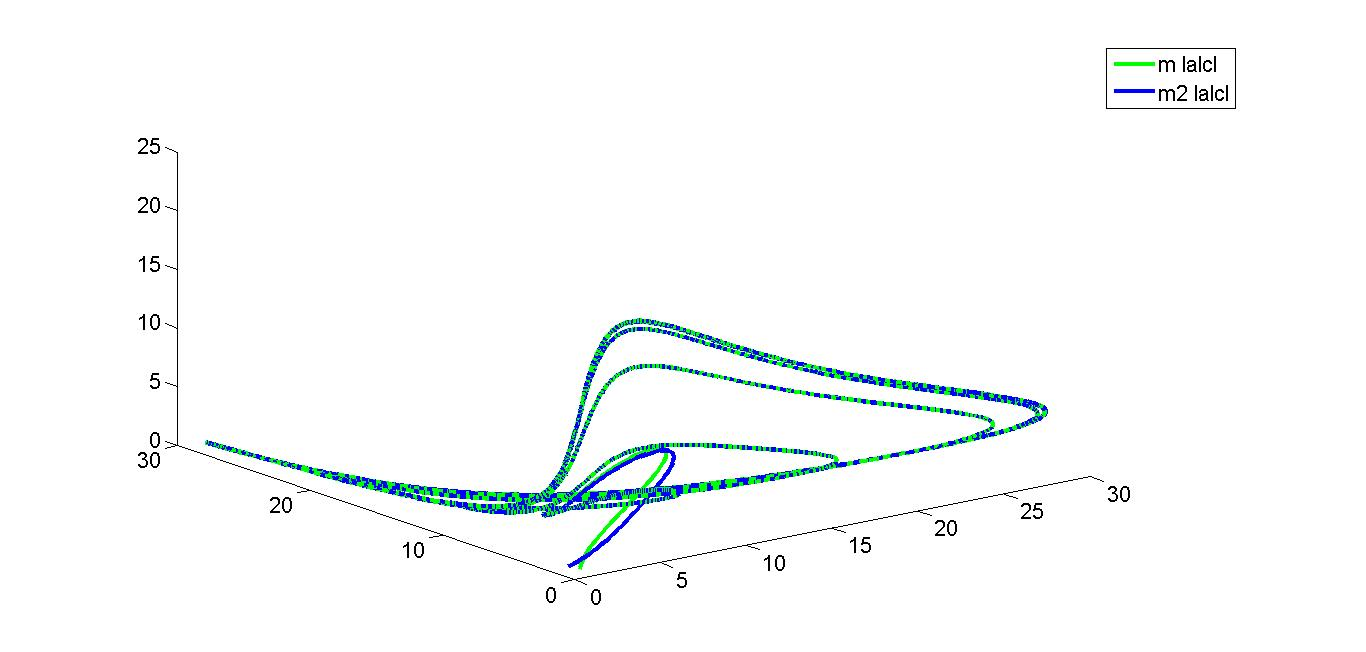
\includegraphics[width=12cm]{coupled3d}
 	   	\caption{The coupled case }
 	   \end{figure}
 	   \begin{figure}[H]
 	   	\centering
 	   	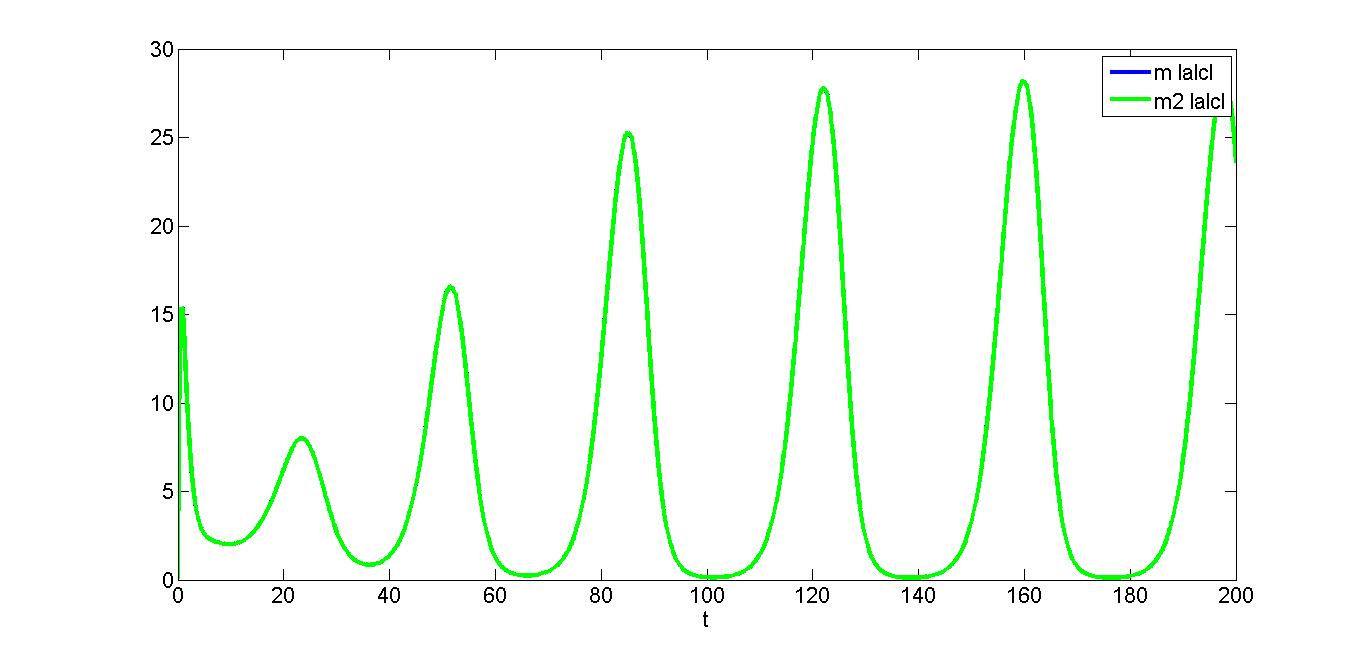
\includegraphics[width=12cm]{coup_osc}
 	   	\caption{Converged oscillations in the uncoupled case}
 	   \end{figure} 	   	   	
\section{Systems biology and network motifs}
Let us start with Shen-Orr's paper and try to model those odes before.
\begin{lstlisting}[style=MyPythonstyle]
import scipy.integrate as si
import numpy as np
import matplotlib.pyplot as plt

#The forcing (X)
def sigm(t):
	if 2<t <6 :
		f=1
	else:
		f=0  
	return f
	
#The function F	
def sigm2(t):
	if 0.5<t  :
		f=1
	else:
		f=0  
	return f 
	
#The derivative		
def ode(y, t):
	return [sigm(t)-y[0],sigm2(y[0])*sigm(t)-y[1]]
	
t  = np.linspace(0, 10, 1000) 
yzero = np.array([0.,0.])
y = si.odeint(ode, yzero, t)

#Plots
fig = plt.figure()
ax = fig.add_subplot(111)
plt.plot(t, y[:,0], label='y')
plt.plot(t, y[:,1], label='z')
handles, labels = ax.get_legend_handles_labels()
ax.legend(handles, labels)
plt.show()
\end{lstlisting}
 	   \begin{figure}[H]
 	   	\centering
 	   	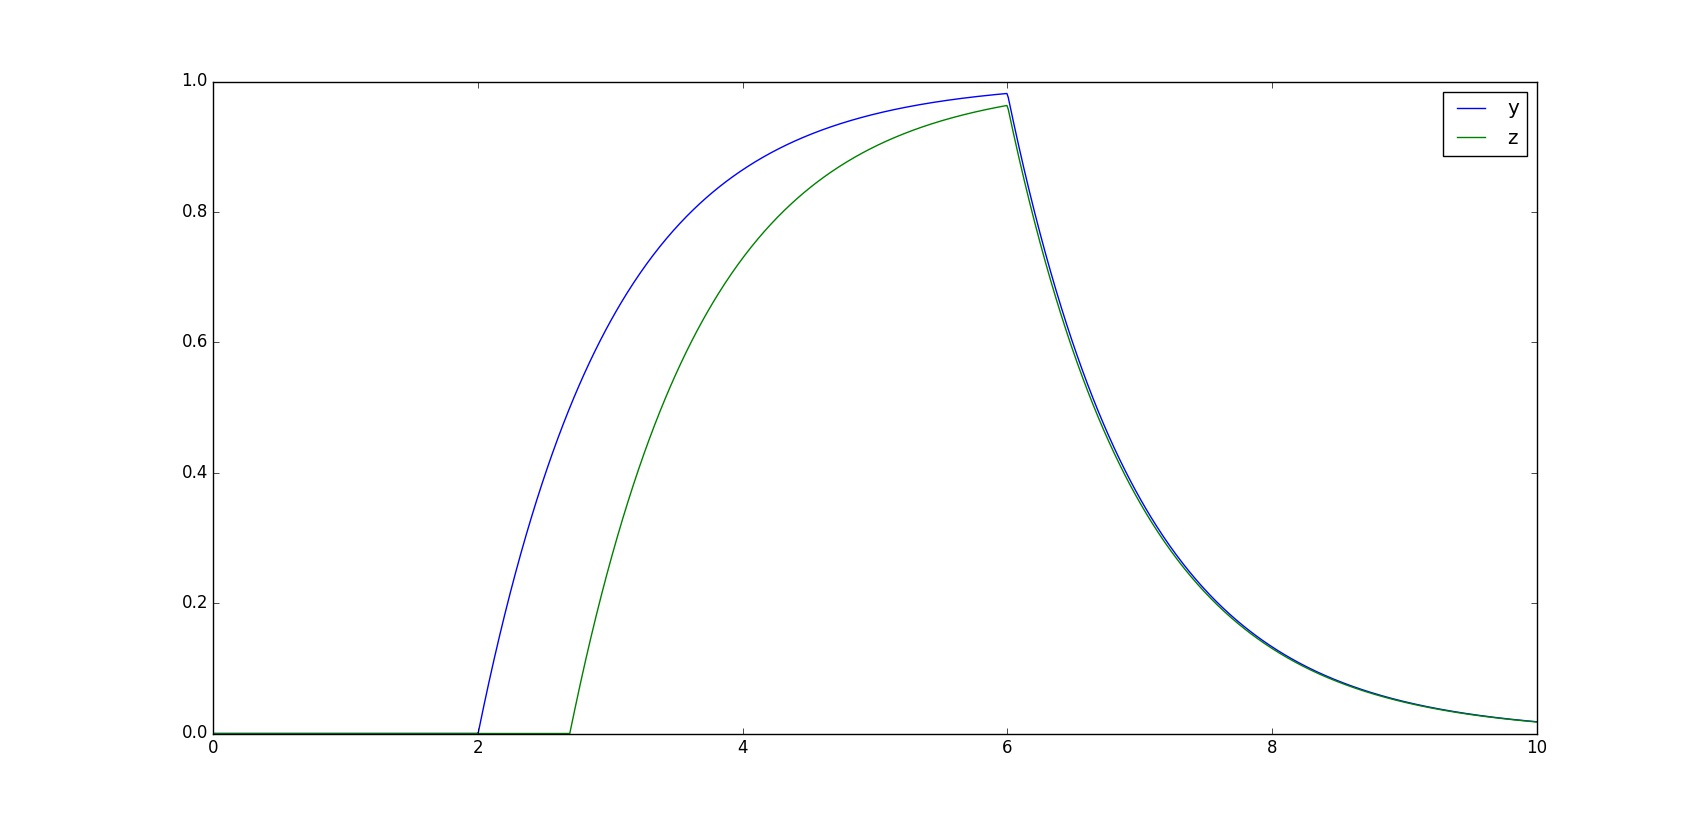
\includegraphics[width=12cm]{Shennor}
 	   	\caption{Shen-Orr odes}
 	   \end{figure}	
This matches quite well with the figure 2a in the paper.

However, Alon's results appears to follow a different path after the forcing is over. In fact, at t=6, the graphs seem to continue on unaffected. After  doing a few trials and errors, we get graphs like the ones below.
 	   \begin{figure}[H]
 	   	\centering
 	   	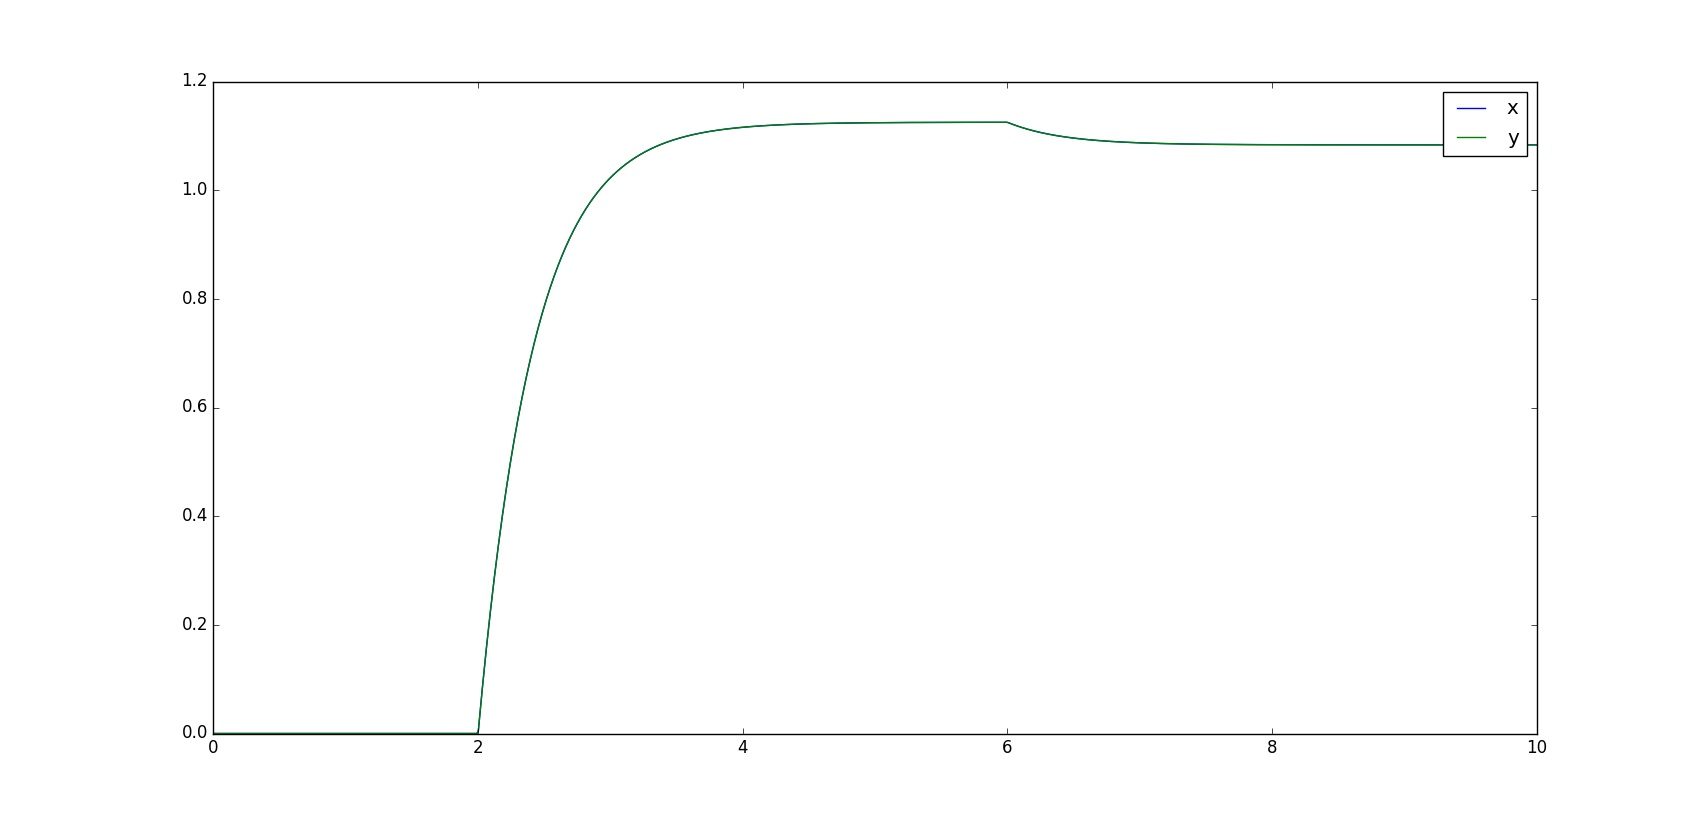
\includegraphics[width=12cm]{Trial}
 	   	\caption{Trial and error graph}
 	   \end{figure}
Alon's graphs appears to increase and don't seem to have the discontinuity at t=6.
For this to happen, the derivative at t=6 must not have two values. 
Let p refer to the concentrations of both X and Y since they are identical.

Left derivative at 6 = right derivative at 6.
\[tF(p)F(x=6^-)+F(x=6^-)-bp=tF(p)F(x=6^+)+F(x=6^+)-bp\]
\[tF(p)+1-bp=-bp\]  
\[tF(p)+1=0\]  
\[t=-1\]
For the derivative to be single valued at 6, the coefficient of the non-linear term has to be -1. Plugging this in, we attempt to get new insights.
 	\begin{lstlisting}[style=MyPythonstyle]
import scipy.integrate as si
import numpy as np
import matplotlib.pyplot as plt

#The forcing (X)
def sigm(t):
	if 2<t <6 :
		f=1
	else:
		f=0  
	return f

#The function F	
def sigm2(t):
	if 0.0<t  :
		f=1
	else:
		f=0  
	return f 

#The derivative    
def ode(y, t):
	return[-1.*sigm2(y[1])*sigm(t)+sigm(t)-0.4*y[0],
	-1.*sigm2(y[0])*sigm(t)+sigm(t)-0.4*y[1]]

t  = np.linspace(0, 10, 1000) 
yzero = np.array([0.,0.])
y = si.odeint(ode, yzero, t)

#Plots
fig = plt.figure()
ax = fig.add_subplot(111)
plt.plot(t, y[:,0], label='y')
plt.plot(t, y[:,1], label='z')
handles, labels = ax.get_legend_handles_labels()
ax.legend(handles, labels)
plt.show() 
 	\end{lstlisting}
 	   \begin{figure}[H]
 	   	\centering
 	   	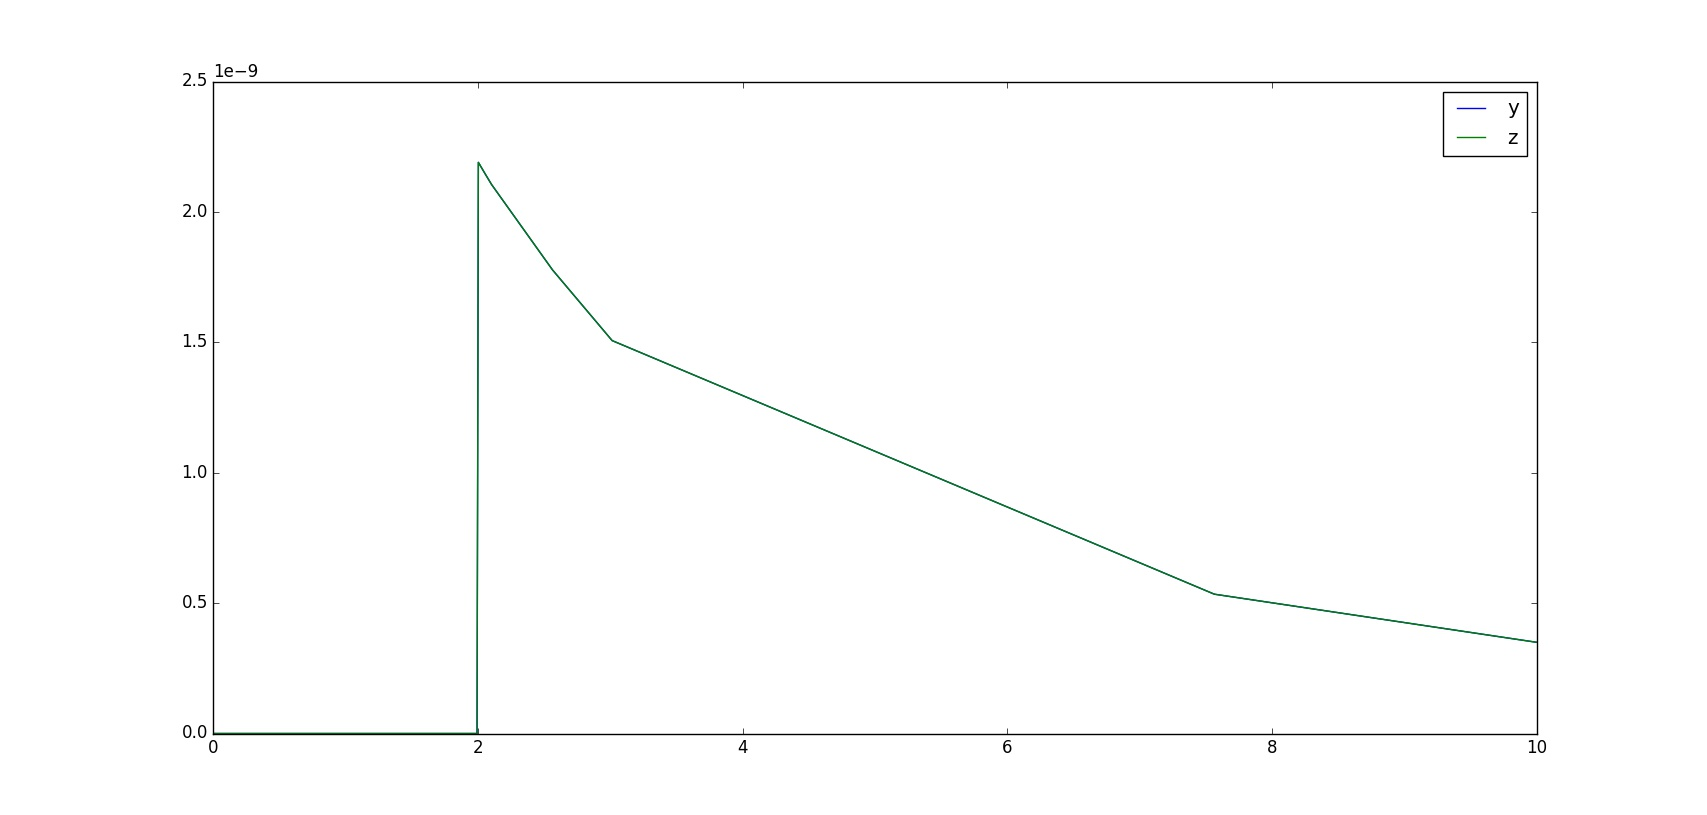
\includegraphics[width=12cm]{disc}
 	   	\caption{Cost of making the derivative exist}
 	   \end{figure}	 	
The derivative is continuous at 6 but this is far from the graph we want and thus, we assume that there is a jump in the derivative at t=6. So, each term in the derivative has an F(z) part. Using this, we can model our equations as
\[\frac{dx}{dt} = F(z)F(x)+F(z)-xF(z)\] 	
\[\frac{dy}{dt} = F(z)F(y)+F(z)-yF(z)\] 
Where,
\[\]
Scaling appropriately, we plug it into the code.
 	\begin{lstlisting}[style=MyPythonstyle]
import scipy.integrate as si
import numpy as np
import matplotlib.pyplot as plt

#F(z)
def sigm(t):
	if 2<t <6 :
		f=1
	else:
		f=0  
	return f

#F(x)/F(y)	
def sigm2(t):
	if 0.0<t  :
		f=1
	else:
		f=0  
	return f 
		
def ode(y, t):
	return[0.5*sigm2(y[1])*sigm(t)+0.5*sigm(t)-y[0]*sigm(t),
	0.5*sigm2(y[0])*sigm(t)+0.5*sigm(t)-y[1]*sigm(t)]

t  = np.linspace(0, 10, 1000) 
yzero = np.array([0.,0.])
y = si.odeint(ode, yzero, t)

#Plots
fig = plt.figure()
ax = fig.add_subplot(111)
plt.plot(t, y[:,0])
plt.plot(t, y[:,1])
plt.plot(t, y[:,0], label='x')
plt.plot(t, y[:,1], label='y')
handles, labels = ax.get_legend_handles_labels()
ax.legend(handles, labels)
plt.show() 
 	\end{lstlisting}
 	   \begin{figure}[H]
 	   	\centering
 	   	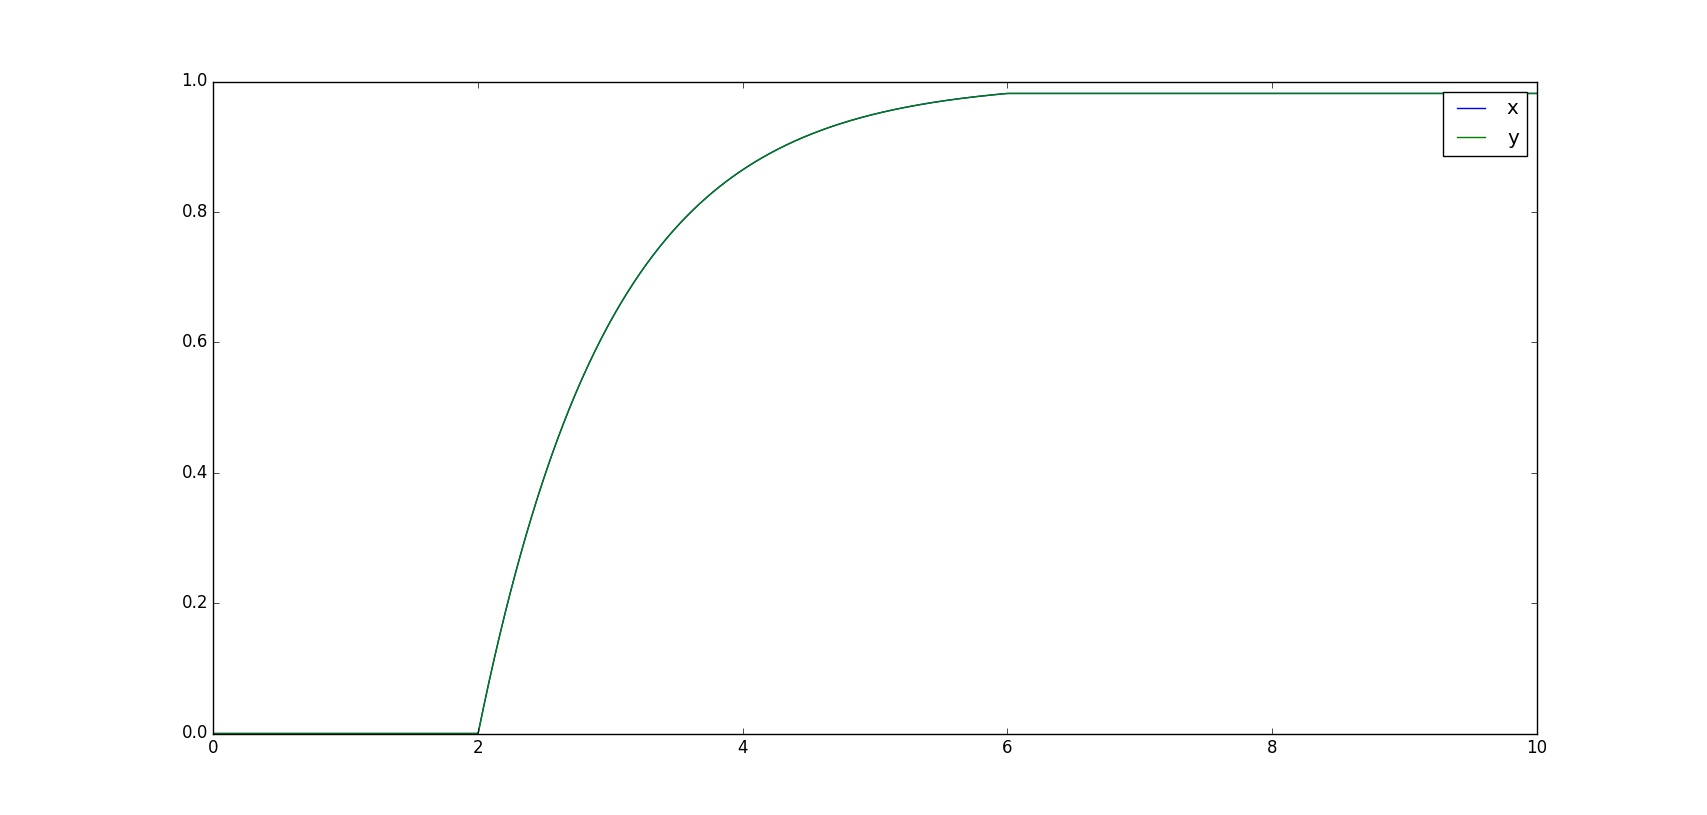
\includegraphics[width=12cm]{motif}
 	   	\caption{Double positive feedback loop}
 	   \end{figure}	

Similarly, for the negative feedback loop,
\[\frac{dx}{dt} = F(z)F(x)+F(z)-xF(z)\] 	
\[\frac{dy}{dt} = F(z)F(y)-F(z)-yF(z)\] 

 	\begin{lstlisting}[style=MyPythonstyle]
import scipy.integrate as si
import numpy as np
import matplotlib.pyplot as plt

#F(z)
def sigm(t):
	if 2<t <6 :
		f=1
	else:
		f=0  
	return f

#F(x)/F(y)
def sigm2(t):
	if 0.0<t  :
		f=1
	else:
		f=0  
	return f 

def ode(y, t):
	return[0.5*sigm2(y[1])*sigm(t)+0.5*sigm(t)-y[0]*sigm(t),
	1*sigm2(y[0])*sigm(t)-sigm(t)-y[1]*sigm(t)]

t  = np.linspace(0, 10, 1000) 
yzero = np.array([0.,0.])
y = si.odeint(ode, yzero, t)

#Plots
fig = plt.figure()
ax = fig.add_subplot(111)
plt.plot(t, y[:,0])
plt.plot(t, y[:,1])
plt.plot(t, y[:,0], label='x')
plt.plot(t, y[:,1], label='y')
handles, labels = ax.get_legend_handles_labels()
ax.set_ylim([-0,1.10])
ax.legend(handles, labels)
plt.show() 
 	\end{lstlisting} 
 	
 	   \begin{figure}[H]
 	   	\centering
 	   	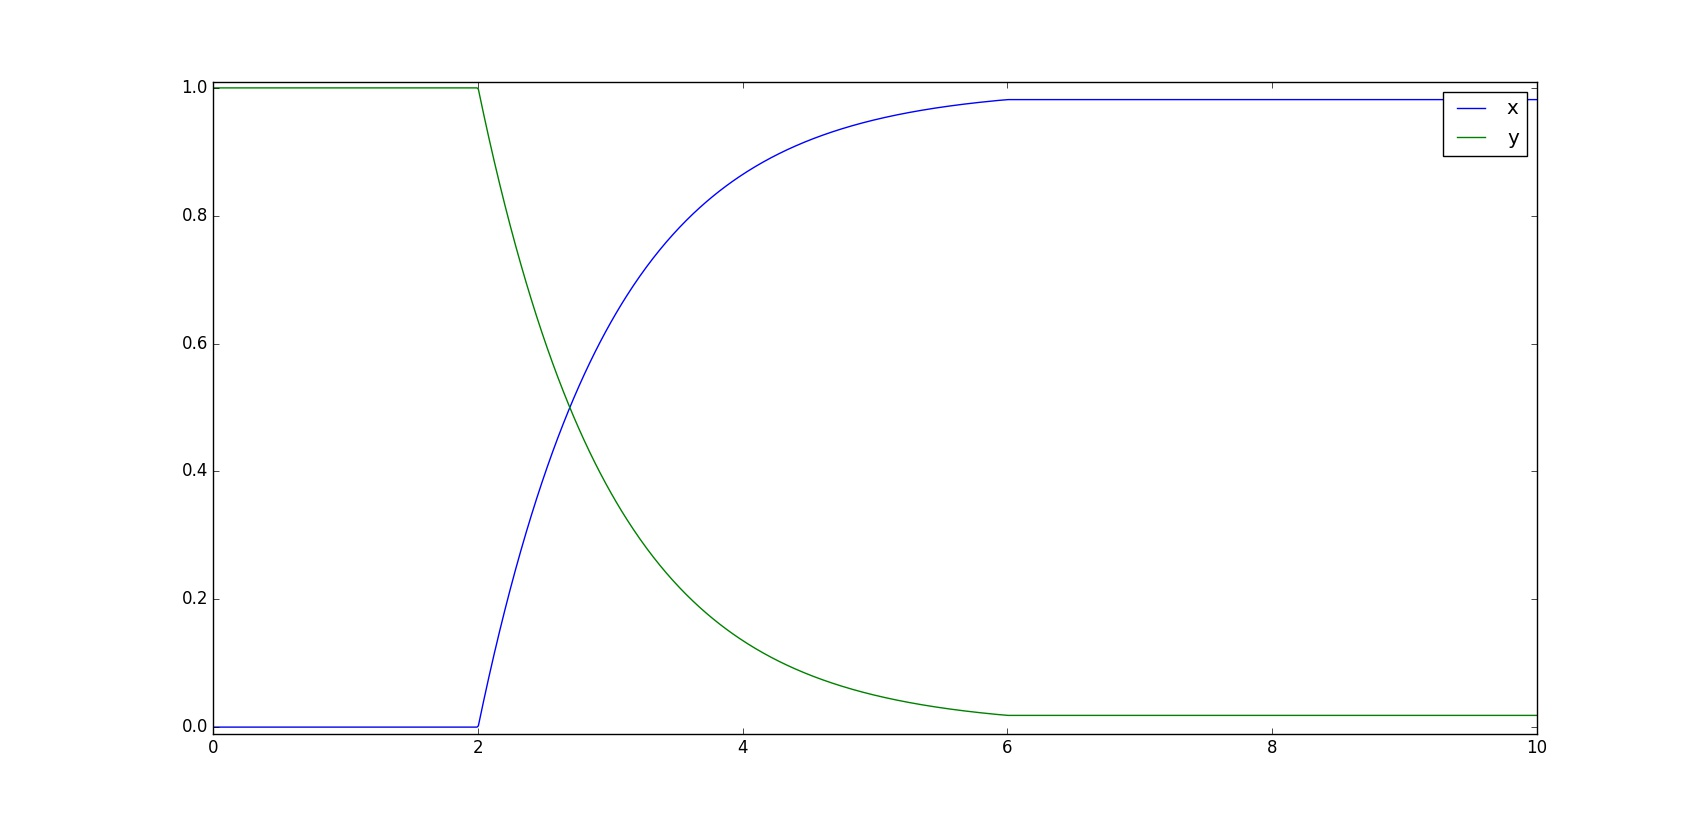
\includegraphics[width=12cm]{motif2}
 	   	\caption{Double negative feedback loop}
 	   \end{figure} 		
\section{Python}
 \begin{itemize}
 	\item  Exercise : Random guassian distribution
 	\begin{lstlisting}[style=MyPythonstyle]
import numpy as np
m= 5
s = np.sqrt(2)
p=np.random.normal(5,s,100)
print(np.mean(p))
print(np.var(p))
 	\end{lstlisting}
 The answer often varies but for one instance, mean was 5.09347742313 and the variance was 1.94676873609.
 	\item Exercise 2: Solving an ode
 	\begin{lstlisting}[style=MyPythonstyle]
import scipy.integrate as si
import numpy as np
import matplotlib.pyplot as plt

def ode(y, t):
   yprime = y
   return yprime


#lrun    ODE solving example: .

t = np.arange(0, 10.01, .01)  #x time points on which to solve
yzero = np.array([1.])

y = si.odeint(ode, yzero, t)
print (y)
plt.plot(t, y)
plt.xlabel('t')
plt.ylabel('y')
plt.title('The ode')
plt.show()     	
 	\end{lstlisting} 
 	   \begin{figure}[H]
 	   	\centering
 	   	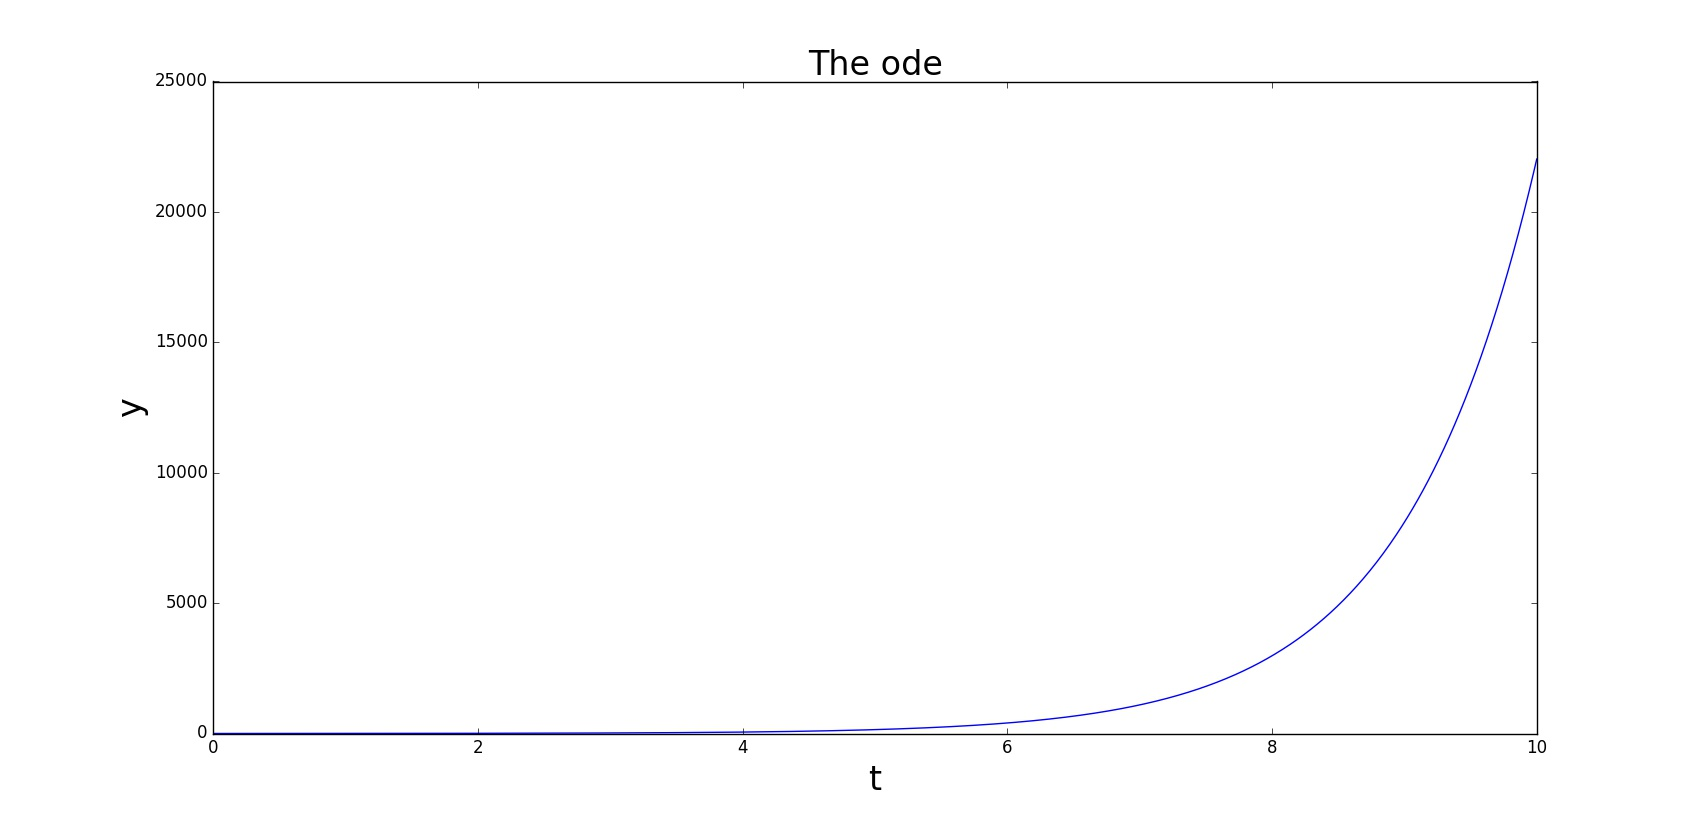
\includegraphics[width=12cm]{figure_1}
 	   	\caption{Exercise 2}
 	   \end{figure}	
 	\end{itemize}
 	
     
\end{document}